\begin{center}
\Huge
	Anvendelser af integraler
\end{center}

\section*{Bevægelseslære}
\stepcounter{section}

I forbindelse med vores forløb om differentialregning introducerede vi ganske kort følgende sammenhæng mellem accelerationen, hastigheden og forskydningen af et objekt. Navnligt for forskydningsfunktionen $d$, hastighedsfunktionen
$v$ og accelerationen $a$, at 
\begin{align*}
	d'(t) = v(t)	
\end{align*}
samt
\begin{align*}
	d''(t) = v'(t) = a(t). 
\end{align*}
Vi må derfor tilsvarende kunne bevæge os i den modsatte retning ved at integrere. Dette illustreres på Figur \ref{fig:kinematik}
\begin{figure}[H]
	\centering
	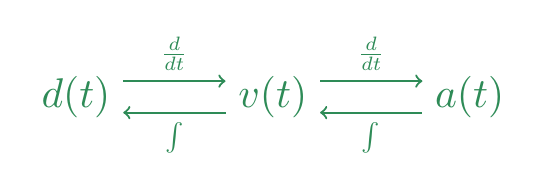
\begin{tikzpicture}
		\node[color = SeaGreen, scale = 1.5] at (0,0) {$d(t)$};
		\draw[color = SeaGreen, ->, thick] (0.6,0.2) -- (1.9,0.2) node[midway, anchor = south] {$\frac{d}{dt}$}; 
		\node[color = SeaGreen, scale = 1.5] at (2.5,0) {$v(t)$};
		\draw[color = SeaGreen, ->, thick] (3.1,0.2) -- (4.4,0.2) node[midway, anchor = south] {$\frac{d}{dt}$}; 
		\node[color = SeaGreen, scale = 1.5] at (5,0) {$a(t)$};
		%ints
		\draw[color = SeaGreen, <-, thick] (0.6,-0.2) -- (1.9,-0.2) node[midway, anchor = north] {$\int$}; 
		\draw[color = SeaGreen, <-, thick] (3.1,-0.2) -- (4.4,-0.2) node[midway, anchor = north] {$\int$}; 
	\end{tikzpicture}
	\caption{Illustration af sammenhængen mellem forskydning, hastighed og acceleration.}
	\label{fig:kinematik}
\end{figure}
\begin{exa}
	En bil har efter 10 sekunder kørt 300 meter. I det bilen træder på bremsen kører
	den $36\frac{m}{s}$ og bliver udsat for en konstant acceleration på $-6\frac{m}{s^2}$. Vi ønsker at finde afstanden, 
	bilen har kørt, når den holder stille. 
	Vi finder først hastighedsfunktionen $v(t)$.
	\begin{align*}
		v(t) = \int -6 dt = -6t + k,	
	\end{align*}
	og da $v(0) = 36$, så må det gælde, at 
	\begin{align*}
		v(0) = -6\cdot 0 + k = 36 \Leftrightarrow k = 36.
	\end{align*}
	Vi kan nu finde forskydningsfunktionen ved igen at integrere.
	\begin{align*}
		d(t) = \int -6t + 36 dt &= \frac{-6}{2}t^2 + 36t + c \\
		&= -3t^2 + 36t + c.
	\end{align*}
	Vi finder nu tallet $c$ som før.
	\begin{align*}
		d(0) = -3\cdot 0^2 + 36\cdot 0 + c = 300 \Leftrightarrow 300 = c
	\end{align*}
	Vi har derfor forskydningsfunktionen
	\begin{align*}
		d(t) = -3t^2 + 36t + 300,
	\end{align*}
	men mangler tidspunktet, hvor hastigheden er 0, så vi bruger $v$, og får
	\begin{align*}
		v(t) = 0 \Leftrightarrow -6t = 36 \Leftrightarrow t = 6s.
	\end{align*}
	Der går altså 6 sekunder før bilen stopper. Dette sættes nu ind i forskydningsfunktionen, som giver os
	\begin{align*}
		d(6) = -3\cdot 6^2 + 36\cdot 6 + 300 = -108 + 216 + 300 = 408m.
	\end{align*}
	Bilen har altså flyttet sig 408 meter, når den står stille. 108 af disse er forløbet under nedbremsningen. 
\end{exa}

\section*{Gennemsnit af funktioner}
\stepcounter{section}

Skal vi bestemme et gennemsnit af højden af alle i en klasse, vil vi måle højden på alle i klassen, summere det og dele med antallet af studerende i klassen. Vi kan generalisere dette til kontinuerte funktioner ved hjælp af integraler.

\begin{defn}
Gennemsnittet af en kontinuert funktion $f$ på intervallet $[a,b]$ defineres som integralet
\begin{align*}
I = \frac{1}{b-a}\int_a^bf(x)dx.
\end{align*}
\end{defn}

\begin{exa}
Koncentrationen af en bestemt type partikel i en by kan beskrives ved eksponentialfunktionen
\begin{align*}
f(x) = 22.145\cdot 1.32^x,
\end{align*}
hvor $f$ er i ppm og $x$ er i år efter år 2000. Ønsker vi at bestemme den gennemsnitlige koncentration fra år 2002 til år 2010, så kan vi bestemme det som
\begin{align*}
I = \frac{1}{10-2}\int_2^{10}22.145\cdot 1.32^x dx, 
\end{align*}
som med et CAS-værktøj bestemmes til at være
$$I = 142.751 ppm.$$
Dette vil altså være den gennemsnitlige partikelkoncentration henover de 8 år.
\end{exa}

\subsection*{Opgave 1 (Med Maple)}

Et kommercielt fly har en typisk landingshastighed på omkring $70 \frac{m}{s}$, og det bruger ca. 20 sekunder på at standse.

\begin{enumerate}[label=\roman*)]
	\item Bestem accelerationen for et fly fra det lander på landingsbanen til det står stille, hvis vi antager, at 
	accelerationen er konstant. 
	\item Bestem den afstand, flyet bruger på at standse. 
\end{enumerate}

\subsection*{Opgave 2 (Med Maple)}

Tyngdeaccelerationen på jorden er alt afhængigt af sted omtrent $9.81\frac{m}{s^2}$. 
\begin{enumerate}[label=\roman*)]
	\item Bestem hastigheden af en faldskærmsudspringer to sekunder efter et udspring, hvis vi ser bort fra luftmodstand.
	\item Bestem afstanden udspringeren vil være faldet efter 3 sekunder. 
\end{enumerate}

\subsection*{Opgave 3 (Med Maple)}
En funktion $f$ er givet ved
\begin{align*}
	f(x) = 2x + 5
\end{align*}
\begin{enumerate}[label=\roman*)]
	\item Bestem den gennemsnitlige funktionsværdi på intervallet $[0,4]$. 
\end{enumerate}

\subsection*{Opgave 4 (Med Maple)}
Forskydningen af en bil er givet ved funktionen
\begin{align*}
	d(t) = 0.5t^2 + 25t + 100,
\end{align*}
hvor $t$ er den forløbne tid i sekunder og $d$ er forskydningen i $m$.
\begin{enumerate}[label=\roman*)]
	\item Bestem hastighedsfunktionen $v(t)$.
	\item Bestem den gennemsnitlige hastighed på intervallet $[5,20]$. 
\end{enumerate}

\subsection*{Opgave 5 (Med Maple)}
Siden 1996 har Danmarks udledning af CO$_2$'ækvivalenter kunnet beskrives approksimativt ved
\begin{align*}
	f(t) = 99.7\cdot 0.97^t,
\end{align*}
hvor $t$ betegner antal år siden 1996 og $f$ betegner udledningen i CO$_2$-ækvivalenter i mio. tons CO$_2$.
\begin{enumerate}[label=\roman*)]
	\item Bestem CO$_2$-udledningen i år $1996$ og $2026$.
	\item Bestem den gennemsnitlige udledning per år fra $1996$ til $2026$. 
\end{enumerate}

\subsection*{Opgave 6 (Med Maple)}
En funktion $f$ er givet ved
\begin{align*}
	f(x) = x^3 - ax + 4
\end{align*}
\begin{enumerate}[label=\roman*)]
	\item Bestem tallet $a$, så den gennemsnitlige funktionsværdi på $[-2,7]$ er $10$.
	\item Bestem de værdier for $b$, så den gennemsnitlige funktionsværdi på $[b,11]$ er $20$.
\end{enumerate}

\subsection*{Opgave 7 (Med Maple)}
Profilen af en hængebro er indlejret i et koordinatsystem. Kablet mellem pylonerne tager form som grafen for polynomiet $p$ givet ved
\begin{align*}
	p(x) = 0.00028125x^2 -0.45x + 250,
\end{align*}
hvor $p$ er højden af kablet, og $x$ er den vandrette afstand fra broens venstre pylon. Alle enheder er i meter.
\begin{enumerate}[label=\roman*)]
	\item Tegn grafen for $p$ på intervallet $[0,1800]$. 
	\item Bestem højden af de to pyloner. (De er lige høje).
	\item Bestem afstanden mellem de to pyloner. 
	\item Bestem længden af kablet.
\end{enumerate}

\subsection*{Opgave 8}
Vi skal bevise, at volumen af en kugle med radius er givet ved
\begin{align*}
	\frac{4}{3}\pi r^3.
\end{align*}
\begin{enumerate}[label=\roman*)]
	\item Udnyt, at cirklens ligning er givet ved $x^2 + y^2 = r^2$, hvor $r$ er cirklens radius til at bestemme en 
	forskrift for cirklens øverste halvbue. (Vink: Isolér $y$ i udtrykket.)
	\item Bestem volumen af omdrejningslegemet for den øverste halvbue af cirklen. 
\end{enumerate}